\documentclass[a4paper,]{article}
\usepackage{lmodern}
\usepackage{amssymb,amsmath}
\usepackage{ifxetex,ifluatex}
\usepackage{fixltx2e} % provides \textsubscript
\ifnum 0\ifxetex 1\fi\ifluatex 1\fi=0 % if pdftex
  \usepackage[T1]{fontenc}
  \usepackage[utf8]{inputenc}
\else % if luatex or xelatex
  \ifxetex
    \usepackage{mathspec}
  \else
    \usepackage{fontspec}
  \fi
  \defaultfontfeatures{Ligatures=TeX,Scale=MatchLowercase}
\fi
% use upquote if available, for straight quotes in verbatim environments
\IfFileExists{upquote.sty}{\usepackage{upquote}}{}
% use microtype if available
\IfFileExists{microtype.sty}{%
\usepackage{microtype}
\UseMicrotypeSet[protrusion]{basicmath} % disable protrusion for tt fonts
}{}
\usepackage[margin=1in]{geometry}
\usepackage{hyperref}
\hypersetup{unicode=true,
            pdftitle={Onshore wind and the likelihood of planning acceptance: learning from a Great Britain context},
            pdfauthor={Michael Harper, Ben Anderson, Patrick James, AbuBakr Bahaj},
            pdfborder={0 0 0},
            breaklinks=true}
\urlstyle{same}  % don't use monospace font for urls
\usepackage{longtable,booktabs}
\usepackage{graphicx,grffile}
\makeatletter
\def\maxwidth{\ifdim\Gin@nat@width>\linewidth\linewidth\else\Gin@nat@width\fi}
\def\maxheight{\ifdim\Gin@nat@height>\textheight\textheight\else\Gin@nat@height\fi}
\makeatother
% Scale images if necessary, so that they will not overflow the page
% margins by default, and it is still possible to overwrite the defaults
% using explicit options in \includegraphics[width, height, ...]{}
\setkeys{Gin}{width=\maxwidth,height=\maxheight,keepaspectratio}
\IfFileExists{parskip.sty}{%
\usepackage{parskip}
}{% else
\setlength{\parindent}{0pt}
\setlength{\parskip}{6pt plus 2pt minus 1pt}
}
\setlength{\emergencystretch}{3em}  % prevent overfull lines
\providecommand{\tightlist}{%
  \setlength{\itemsep}{0pt}\setlength{\parskip}{0pt}}
\setcounter{secnumdepth}{5}
% Redefines (sub)paragraphs to behave more like sections
\ifx\paragraph\undefined\else
\let\oldparagraph\paragraph
\renewcommand{\paragraph}[1]{\oldparagraph{#1}\mbox{}}
\fi
\ifx\subparagraph\undefined\else
\let\oldsubparagraph\subparagraph
\renewcommand{\subparagraph}[1]{\oldsubparagraph{#1}\mbox{}}
\fi

%%% Use protect on footnotes to avoid problems with footnotes in titles
\let\rmarkdownfootnote\footnote%
\def\footnote{\protect\rmarkdownfootnote}

%%% Change title format to be more compact
\usepackage{titling}

% Create subtitle command for use in maketitle
\newcommand{\subtitle}[1]{
  \posttitle{
    \begin{center}\large#1\end{center}
    }
}

\setlength{\droptitle}{-2em}
  \title{Onshore wind and the likelihood of planning acceptance: learning from a
Great Britain context}
  \pretitle{\vspace{\droptitle}\centering\huge}
  \posttitle{\par}
  \author{Michael Harper, Ben Anderson, Patrick James, AbuBakr Bahaj}
  \preauthor{\centering\large\emph}
  \postauthor{\par}
  \date{}
  \predate{}\postdate{}

\usepackage{booktabs}
\usepackage{longtable}
\usepackage{array}
\usepackage{multirow}
\usepackage[table]{xcolor}
\usepackage{wrapfig}
\usepackage{float}
\usepackage{colortbl}
\usepackage{pdflscape}
\usepackage{tabu}
\usepackage{threeparttable}
\usepackage[normalem]{ulem}

\usepackage{setspace}\doublespacing

\usepackage{amsthm}
\newtheorem{theorem}{Theorem}[section]
\newtheorem{lemma}{Lemma}[section]
\theoremstyle{definition}
\newtheorem{definition}{Definition}[section]
\newtheorem{corollary}{Corollary}[section]
\newtheorem{proposition}{Proposition}[section]
\theoremstyle{definition}
\newtheorem{example}{Example}[section]
\theoremstyle{definition}
\newtheorem{exercise}{Exercise}[section]
\theoremstyle{remark}
\newtheorem*{remark}{Remark}
\newtheorem*{solution}{Solution}
\begin{document}
\maketitle

\subsection*{Abstract}\label{abstract}
\addcontentsline{toc}{subsection}{Abstract}

Geospatial modelling is extensively used to identify suitable sites for
the installation of onshore wind turbines. However, there are concerns
that such approaches do not accurately consider the social issues
surrounding such projects, resulting in large numbers of projects
subsequently being rejected at planning permission. Using the location
of 1691 historic wind turbine planning applications in Great Britain,
this paper explores whether the planning success of proposed wind
turbine projects can be predicted using a range of geospatial, social
and political parameters. The results indicate that the size of the
project, percentage of the local population with high levels of
qualifications, the average age, and the proximity to existing wind
turbines are key influences affecting planning approval. The paper
demonstrates that quantitatively linking regional social and political
data enhances the assessment of the planning outcome of wind turbines,
and highlights that geospatial parameters are in themselves limited in
identifying the suitability of sites. This suggests that existing policy
is\ldots{}

\subsection*{Keywords}\label{keywords}
\addcontentsline{toc}{subsection}{Keywords}

Onshore Wind, Logistic Regression, Planning, Demographics, Great
Britain, GIS

\textbf{Word Count}: 5134

\section{Introduction}\label{introduction}

Increased environmental concern and issues surrounding security of
energy supply have led to a global drive to develop renewable energy
systems. Over \$40 billion is invested annually within the European
Union, with this figure expected to exceed \$60 billion by 2020
{[}\protect\hyperlink{ref-UNEP2016}{1}{]}.

Whilst many renewable energy technologies are available, onshore wind is
is one of the most established technologies and offers one of the
least-cost options for renewable energy supply. For example, the cost
projections for new onshore wind projects in the United Kingdom in 2020
are projected to be between £47-76/MWh, a price which competes with
conventional fossil-fuel technologies
{[}\protect\hyperlink{ref-DBIES2016}{2}{]}. This economic viability is
coupled with a high resource availability, with the UK and many other
European countries having a large exploitable wind resource
{[}\protect\hyperlink{ref-EuropeanEnvironmentAgency2009}{3}{]}.

Despite the strengths of onshore wind energy, development of the
technology is restricted as there are challenges for proposed projects
to receive planning permission. Proposals often face local opposition,
with visual impact, noise, site access and ecological impacts often
being cited as reasons for objection
{[}\protect\hyperlink{ref-Wolsink2000}{4},\protect\hyperlink{ref-Langer2016}{5}{]}.
These planning challenges are particularly evident in the United
Kingdom, where 52\% of onshore wind projects are refused permission or
are abandoned by the developer
{[}\protect\hyperlink{ref-DECC2016}{6}{]}. As highlighted in Figure
\ref{fig:acceptanceRates}, this rate is signficantly higher than for
other renewable energy technologies in the UK.





\begin{figure}[h]

{\centering 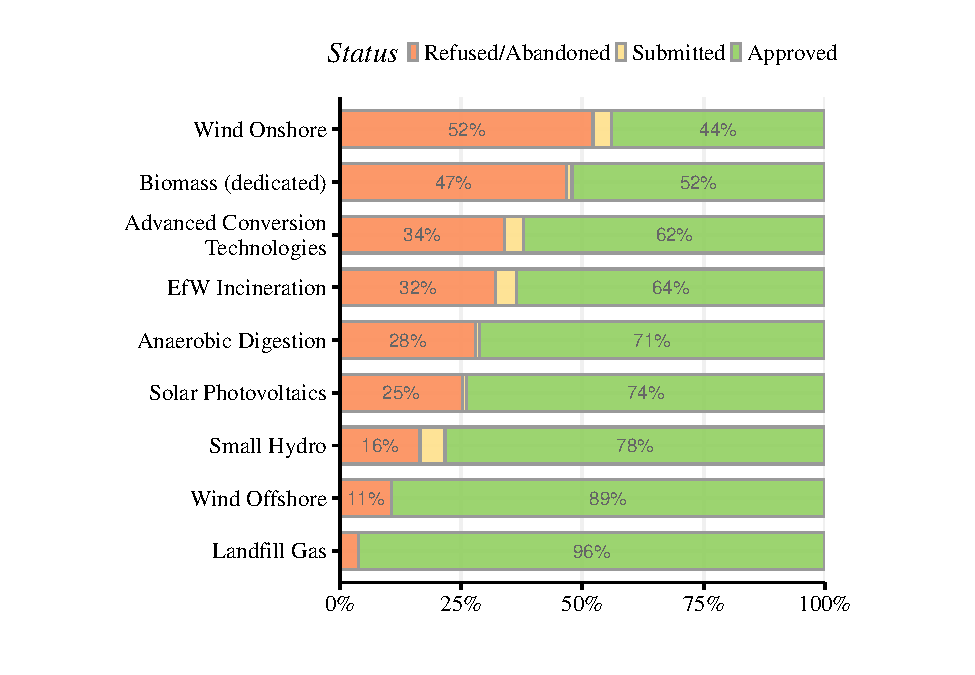
\includegraphics[width=8.8cm]{Paper_files/figure-latex/acceptanceRates-1} 

}

\caption{Acceptance rates of renewable energy projects
within the UK between 1991 and 2017. The Analysis only considers
technologies which have had more than 50 planning applications.}\label{fig:acceptanceRates}
\end{figure}

Whilst planning has been a persistent issue for wind turbines, recent
changes in legislation have severly impacted the development of onshore
wind. Until June 2015, the planning decision for projects greater than
50MW was controlled at a national level. However, this provision was
removed by the \emph{Energy Act 2016} and \emph{Infrastructure Planning
Order 2016}, which provided local authorities with the final say for all
onshore wind energy projects {[}\protect\hyperlink{ref-Smith2016}{7}{]}.
In addition, these wind turbines are only permitted in sites which have
been identified within neighbourhood development plans. These changes
have effectively enabled local communities to be in a position to block
the development of wind turbines in their area.

In addition to changes in planning law, the development of onshore wind
has been further restricted by changes to the financial mechanisms used
to support low-carbon energy in the UK. Onshore wind projects were
removed from the Renewable Obligation scheme on 1st April 2016 {[}@{]},
preventing projects from bidding in the upcoming £557 million (date: )
in subsidies {[}@{]}.

As a result these planning and financial changes, there has been a
dramatic reduction in the development of onshore wind within the UK. In
June 2015, the month the changes in planning were implemented, there
were 133 planning applications for onshore wind, a record high for a
single month {[}\protect\hyperlink{ref-DECC2016}{6}{]}. In contrast, for
the entire year of 2017, there were only 52 planning applications made,
representing only 6\% of the 2015 total. This reduction in planning is
highlighted in Figure \ref{fig:numberApplications}.





\begin{figure}[h]

{\centering \includegraphics[width=8.8cm]{Paper_files/figure-latex/numberApplications-1} 

}

\caption{Number of turbine planning applications
submitted in the United Kingdom per month between January 2013 and
December 2017.}\label{fig:numberApplications}
\end{figure}

Whilst the predicted reduction of cost in onshore wind may overcome the
financial barriers in the long term, the planning changes have act as a
major barrier to increased. This therefore highlights the importance of
considering local communities within the proposals of onshore wind
projects and understanding characteristics which may lead to project
rejection. The UK is not alone in experiencing in encountering
opposition to wind turbine projects
{[}\protect\hyperlink{ref-Langer2016}{5}{]}, but is perhaps unique in
how policy has been restructured to restrict its development.

This paper seeks to understand if existing geospatial modelling of
onshore wind can account for the low levels of acceptance of onshore
wind in the UK (Figure \ref{fig:acceptanceRates}). In addition, existing
social and demographic parameters which can be used to enhance
acceptance rate prediction for the site.

\section{Background}\label{background}

\subsection{Geospatial Modelling}\label{geospatial-modelling}

To assist in the development of onshore wind energy, many methodologies
have been produced to determine site suitability for wind farms.
Development primarily started within the late 1990s
{[}\protect\hyperlink{ref-Voivontas1998}{8},\protect\hyperlink{ref-Baban2001}{9}{]},
and established a structure which has been applied extensively
internationally
{[}\protect\hyperlink{ref-Hansen2005}{10}--\protect\hyperlink{ref-Baseer2017}{25}{]}.
These methodologies combine geospatial modelling with Multi-criteria
Decision Analysis (MCDA) techniques to identify sites which are deemed
suitable for development
{[}\protect\hyperlink{ref-Malczewski2004}{26}{]}.

When determining suitable sites for development, ideal sites are
typically identified as 1) \emph{having high average wind speeds};
\emph{2) not being close to urban areas}; \emph{3) not in protected
landscapes (e.g.~National Parks)}; \emph{4) not close to airports (to
minimise radar interference)}; \emph{5) close to roads for access} and
\emph{6) close to power lines for grid connection}. However, there are
concerns that geospatial parameters in isolation are in themselves
insufficient to explain patterns of development of wind turbines
{[}\protect\hyperlink{ref-VanderHorst2010}{27}{]}. These concerns can be
further supported by the continued reductions in the acceptance of wind
turbine projects in the UK, shown in Figure
\ref{fig:acceptanceRatesWind}, suggesting there is a widening gap
between existing modelling approaches and real world development
patterns.

\begin{figure}[h]

{\centering 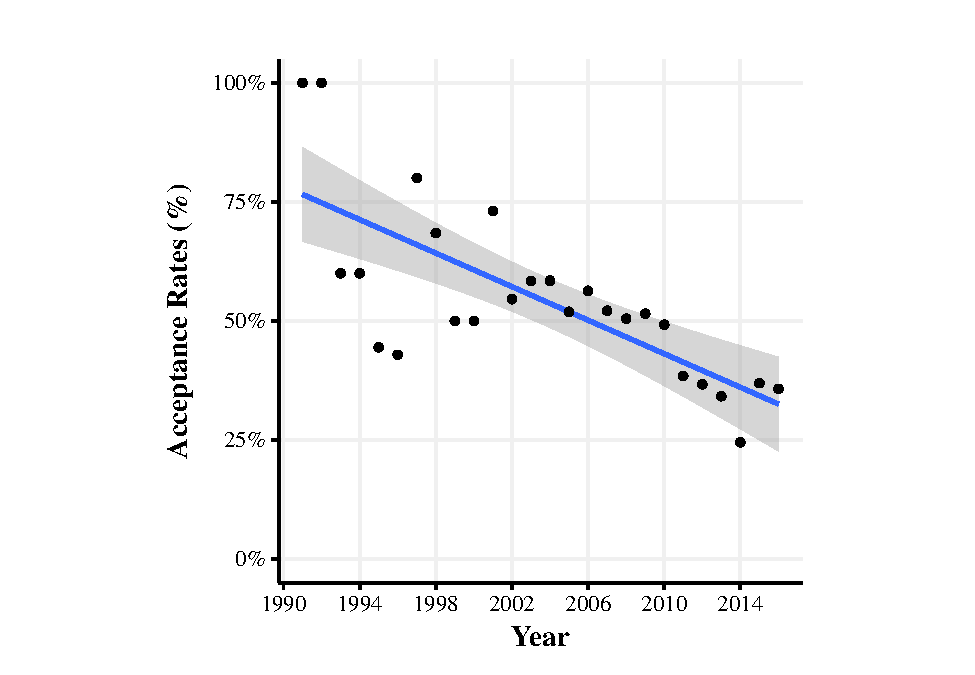
\includegraphics[width=8.8cm]{Paper_files/figure-latex/acceptanceRatesWind-1} 

}

\caption{Annual Average Acceptance rate of wind turbine projects within the UK}\label{fig:acceptanceRatesWind}
\end{figure}

Whilst some studies compare the resulting suitability maps with
locations of operational wind turbines
{[}\protect\hyperlink{ref-Aydin2010}{15},\protect\hyperlink{ref-VanHaaren2011}{16},\protect\hyperlink{ref-Gass2013}{18},\protect\hyperlink{ref-Miller2014}{20},\protect\hyperlink{ref-Watson2015}{22}{]},
these were largely used only as a form of discussion, and the
information was not directly used to develop or revise the models. This
overlooks a valuable contribution that existing sites could provide in
understanding whether there are any spatial development patterns which
can be identified. In particular, Watson
{[}\protect\hyperlink{ref-Watson2015}{22}{]} noted ``\emph{operational
wind farms in South Central England were predominantly located in areas
suggested to be of lower suitability}'', suggesting that the model
inaccurately assesses site suitability in the region.

In situations where there is a large enough sample of similar historical
spatial decisions, an ``\emph{Inverse theory}'' approach can be applied
to determine subjective valuation of criteria by stakeholders
{[}\protect\hyperlink{ref-Cirucci2014}{28}{]}. Compared to the
traditional ``\emph{Forward theory}'' approach of geospatial modelling
(Figure \ref{fig:InverseGIS}a), an inverse approach assesses the
existing spatial distribution of projects to determine the most
influential parameters in determining site success (Figure
\ref{fig:InverseGIS}b). Such an approach has been used successfully
within public health studies
{[}\protect\hyperlink{ref-Brody2002}{29}--\protect\hyperlink{ref-Garcia-Ayllon2013}{32}{]}
and infrastructure location decision-making
{[}\protect\hyperlink{ref-USEPA2002}{33},\protect\hyperlink{ref-Cirucci2015}{34}{]}
to determine optimal sites for development.

\begin{figure}[h]

{\centering 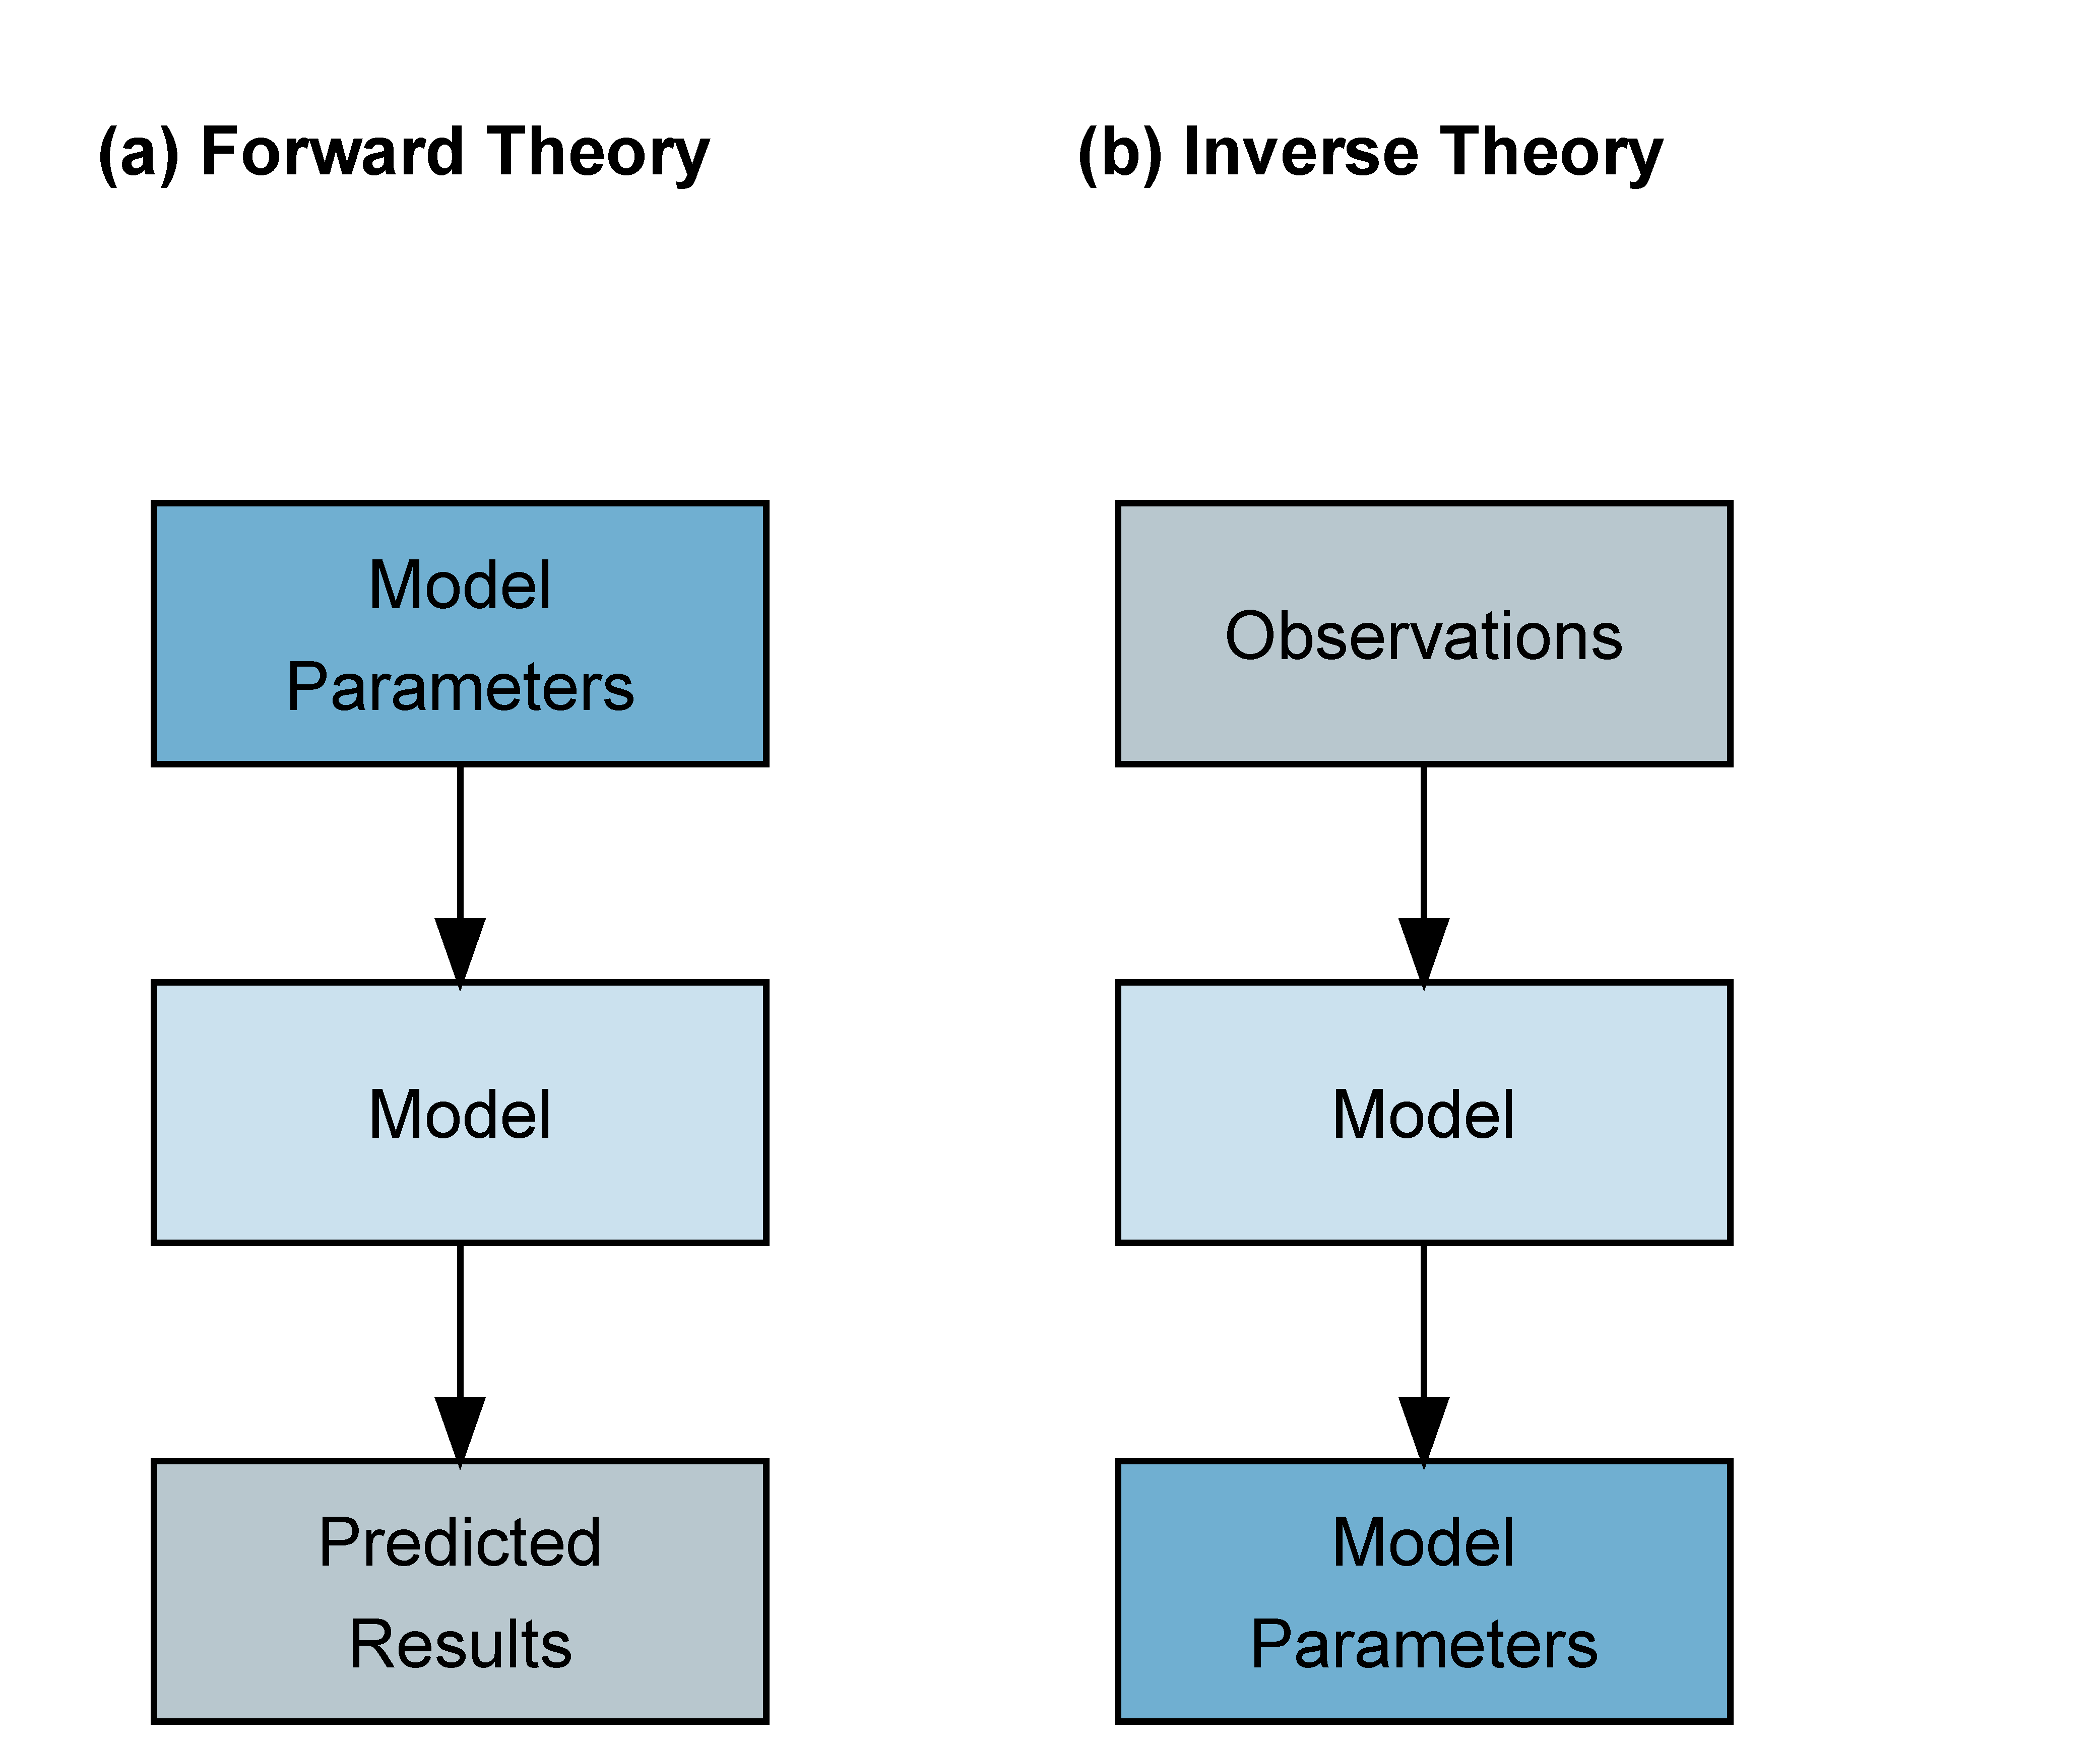
\includegraphics[width=0.5\linewidth]{_figures/InverseGIS/InverseGIS} 

}

\caption{Comparison of Forward and Inverse GIS MCDA model structures}\label{fig:InverseGIS}
\end{figure}

\subsection{Planning Acceptance
Parameters}\label{planning-acceptance-parameters}

The difficulties in receiving planning permission for onshore wind
turbines has prompted research to assess the factors which influence the
public acceptance of onshore wind turbines. It has been highlighted that
the acceptability of wind energy projects is based on more than just
geospatial parameters
{[}\protect\hyperlink{ref-Langer2016}{5},\protect\hyperlink{ref-VanderHorst2010}{27},\protect\hyperlink{ref-Toke2008}{35}{]}.
In a review of 146 journal articles of planning acceptance, perceptions
and attitudes towards wind turbines, Langer et al
{[}\protect\hyperlink{ref-Langer2016}{5}{]} summarised that parameters
can be grouped into three groups 1): \emph{Physical and Environmental};
2) \emph{Pyscho-social} and 3) \emph{Social and Institutional}.

Qualatitive surveys are used to explore potential factors which
influence planning acceptance. A key concept consistently investigated
within empirical research is the \emph{``proximity hypothesis''}, which
states that those living closest to a wind farm will have the most
negative perceptions of it
{[}\protect\hyperlink{ref-Devine-Wright2005}{36},\protect\hyperlink{ref-Warren2005}{37}{]}.
However, attempts to prove this hypothesis have largely proved
unsuccessful, and results have proved conflicting. For example, evidence
from Denmark suggests no link between proximity of residential
properties to the nearest turbine and negative public perceptions, with
suggestions that respondents living closest (i.e.~within 500 metres)
actually had more positive perceptions in comparison with individuals
living away from turbines {[}\protect\hyperlink{ref-Krohn1999}{38}{]}.
This view was further supported by a study in Cornwall, UK, which found
that local communities with visibility of the turbines were generally
more supportive of wind turbines
{[}\protect\hyperlink{ref-Eltham2008}{39}{]}. However, several studies
have reported the opposite relationship
{[}\protect\hyperlink{ref-Meyerhoff2010}{40},\protect\hyperlink{ref-Ladenburg2006}{41}{]},
with the studies finding that negative perceptions increased with
proximity to wind energy developments.

Literature has also sought to understand the potential cumulative
effects that wind turbines have, as projects are frequently refused
planning in regions already containing wind turbines
{[}\protect\hyperlink{ref-Eltham2008}{39},\protect\hyperlink{ref-Strachan2004}{42},\protect\hyperlink{ref-Jones2011}{43}{]}.
However, there has been limited understanding in how neighbouring wind
energy projects may alter the likelihood of nearby wind turbine projects
receiving planning, and current research has focussed on smaller case
studies {[}\protect\hyperlink{ref-Jones2011}{43}{]}.\\
It has been argued within literature that psycho-social factors have
become crucial dimensions to explain how local communities interact
with, and react to, new wind farm developments
{[}\protect\hyperlink{ref-Langer2016}{5}{]}. The effects of
socio-demographic variables on individuals' views of wind farms have
also been studied within literature
{[}\protect\hyperlink{ref-Devine-Wright2005}{36},\protect\hyperlink{ref-Warren2010}{44}{]}.
Age, gender, experience with wind farms, and use of the land and/or
beach were found to be slightly correlated with the attitudes towards
wind power in a Danish study dealing with public perceptions of onshore
or offshore wind energy projects.

At an individual level, empirical findings suggest that political
beliefs are correlated with social acceptance of different low carbon
technologies {[}\protect\hyperlink{ref-Devine-Wright2007}{45}{]}. This
is supported by surveys that indicated that only 62\% of individuals
indicating support for the Conservative party were supportive of new
renewable energy developments, compared to 86\% and 84\% for Labour and
Liberal Democrats respectively
{[}\protect\hyperlink{ref-Populus2005}{46}{]}.

Studies have highlighted that the interaction of developers with local
communities are key indicators of positive planning approval outcomes
{[}\protect\hyperlink{ref-Toke2005}{47}--\protect\hyperlink{ref-Wustenhagen2007}{49}{]}.
Projects which seek greater approval within their plans are generally
more successful than those which are fixed prior to consultation with
the local population.

Finally, the ownership structure of a project has been indicated to be a
significant influence on the level of public acceptance
{[}\protect\hyperlink{ref-Sonnberger2017}{50},\protect\hyperlink{ref-Haggett2006}{51}{]}.
Projects are generally seen as more favourable when owned by local
energy cooperatives than by a large energy company or investor with no
local connections. This reason has been raised to explain the
differences in project success between the United Kingdom and Germany
{[}\protect\hyperlink{ref-Toke2008}{35}{]}.

\subsection{Quantitative Analysis of Turbine
Acceptance}\label{quantitative-analysis-of-turbine-acceptance}

There has been increased use of quantitative analysis to quantify the
effect parameters have on the outcome of wind energy planning outcomes.
Such approaches build upon the understandings provided within the
qualitative analysis explained with Section
\ref{planning-acceptance-parameters}, and aim to provide numerical data
that can be transformed into usable statistics.

Toke {[}\protect\hyperlink{ref-Toke2005}{47}{]} conducted logistic
regression analysis using data collected for 51 wind energy sites within
the UK, and explored how planning outcomes were influenced by the views
of key actors within the planning process of wind energy, including
local councils, planning authorities and landscape protection groups.
The study found that planning acceptance rates were closely associated
with the high level of apprehension about such schemes amongst people
living in the immediate vicinity, highlighting the importance that
social influences have on planning acceptance.

Van der Horst and Toke {[}\protect\hyperlink{ref-VanderHorst2010}{27}{]}
assessed how local characteristics related to the planning outcome of
wind energy projects in England. 117 variables related to education,
health, demography, employment and housing were used and compared with
the planning outcomes for 77 wind energy projects. Univariate regression
analysis was conducted with the Mann-Whitney test being used to analyse
the associations between the planning decision outcome and each of the
independent variables separately. Several strong associations were
identified for planning refusal, including (1) \emph{voter turnout} and
(2) \emph{years of potential life lost}\footnote{Years of potential life
  lost (YPLL) is an estimate of the average years a person would have
  lived if he or she had not died prematurely. It is, therefore, a
  measure of premature mortality.}. The study notes that wind energy
appears to generally be more likely to receive planning permission in
deprived areas, and as previously noted within the review, some
developers were ``\emph{keen to avoid relatively privileged communities
and target areas where people are thought to less likely put up a
fight}'' {[}\protect\hyperlink{ref-VanderHorst2010}{27}{]}. These issues
highlight the potential importance of social parameters in site
selection.

Van Rensburg et al. {[}\protect\hyperlink{ref-VanRensburg20}{52}{]}
utilised adjusted probit regression to assess the relative magnitudes of
association amongst wind farm project planning approval against a range
of 66 variables including project technology, institutional processes
and site endowment. Information was collected from 354 wind farm
applications and planning authority decisions between 1990 and 2011 in
Ireland. The results suggested a range of variables which appeared
significant for planning, including 1) \emph{proximity to Natura 2000
sites}; 2) \emph{sites with high bird sensitivity}; 3) \emph{hub height}
and 4) \emph{project capacity}. In addition, the study noted that
proximity of the nearest dwellings and wind speeds appeared
insignificant, which is counter to the view reported within many
previous studies. Of the variables included within the model, it
concluded a 0.31 predictive confidence value.

\subsection{Combining GIS and Quantitative
Research}\label{combining-gis-and-quantitative-research}

Whilst studies suggest a relationship between demographic and social
data and wind turbine planning acceptance rates, none of geospatial
models reviewed attempted to integrate these into their assessment
beyond the use of proximity buffers around urban areas. It is argued
that this omission fails to fully factor in the social dimension in
terms of its impact on the suitability of sites for development.

Existing quantitative studeis highlight the value which can be provided
by assessing previous planning applications. However, these projects
have been limited in the number of projects considered and the
parameters considered. Responding to calls to combine qualitative and
quantitative research {[}\protect\hyperlink{ref-Langer2016}{5}{]}, this
paper presents analysis which assesses parameters that influence wind
turbine planning outcomes, utilising a range of physical, geographical,
demographic and political parameters.

\section{Material and Methods}\label{material-and-methods}

The overall methodology is highlighted in Figure \ref{fig:Methodology},
with a detailed explanation provided in the following subsections.

\begin{figure}[h]

{\centering 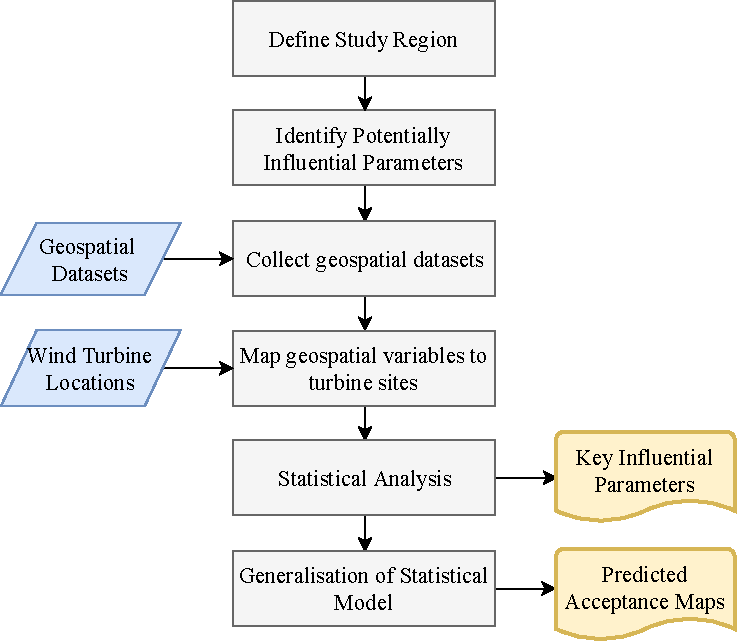
\includegraphics[width=8.8cm]{_figures/Flowchart/ResearchApproach} 

}

\caption{Research methodology}\label{fig:Methodology}
\end{figure}

\subsection{Study Scope}\label{study-scope}

The study was conducted across Great Britain (England, Scotland \&
Wales). These were chosen due to the broadly similar categorisation of
land types, nature designation, data availability and legislation across
these regions {[}\protect\hyperlink{ref-HMGovernment2014}{53}{]}. The
Shetland Islands were excluded from the analysis as their geographic
isolation and distance from mainland Britain created issues in
generalising the model results.

\subsubsection{Wind Turbines Dataset}\label{wind-turbines-dataset}

Information for turbine planning applications was collected through the
Renewable Energy Planning Database (REPD)
{[}\protect\hyperlink{ref-DECC2016}{6}{]} with planning dates between
January 1991 and December 2015 (n=1675). Detailed information for each
planning application includes the location; year of application; number
of turbines; turbine capacity and planning decision. The planning
permission status was summarised to a dichotomous variable for use
within the statistical analysis: 1) \emph{Approved} and 2)
\emph{Refused/Abandoned}. The spatial distribution of these sites is
highlighted in Figure \ref{fig:StudyExtent}.

\begin{figure}[h]

{\centering 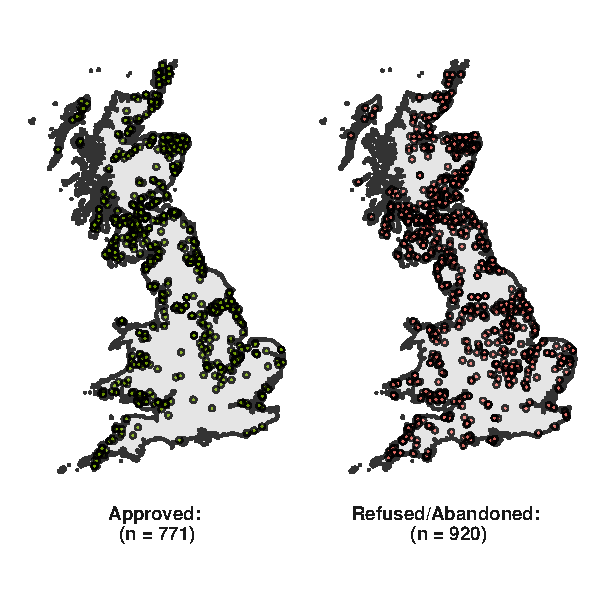
\includegraphics[width=8.8cm]{Paper_files/figure-latex/StudyExtent-1} 

}

\caption{Location of onshore wind energy planning applications used within the study. Location data extracted from the Renewable Energy Planning Database (REPD)}\label{fig:StudyExtent}
\end{figure}

\subsubsection{Model Layers Data}\label{model-layers-data}

Building upon the literature referenced in Section \ref{introduction},
data sources were identified for geospatial and social parameters which
had been indicated to be influence wind turbine planning applications. A
summary of the variables is provided in Table \ref{tab:SummaryTable},
with a full details provided within the Technical Appendix A.

\begin{table}

\begin{threeparttable}
\caption{\label{tab:SummaryTable}Parameters considered within model}
\centering
\begin{tabular}[t]{ll}
\toprule
Category & Variable\\
\midrule
Turbine & Wind Turbine Planning Data\\
 & Turbine Capacity\\
 & Number of Turbines\\
 & Year\\
 & Country\\
Resource & Wind Speed\\
Features & Airports\\
 & Roads\textsuperscript{a}\\
 & Railways\\
 & Urban Areas\\
 & HV Powerlines\textsuperscript{b}\\
 & Military Sites\\
Landscape & Areas of Outstanding Natural Beauty\\
 & National Parks\\
 & Heritage Coast\\
Nature & Special Protection Areas\\
 & National Nature Reserve\\
 & Sites of Special Scientific Interest\\
 & Special Areas of Conservation\\
Geographic & Elevation\\
 & Slope\\
Census & Level of Qualification\textsuperscript{c}\\
 & Age\\
 & Social Grade\textsuperscript{d}\\
 & Tenure\\
Political & Conservatives\\
 & Labour\\
 & Liberal Democrat\\
Proximity & Nearest Turbine (Operational)\\
 & Nearest Turbine (Rejected)\\
\bottomrule
\end{tabular}
\begin{tablenotes}
\small
\item[a] Roads are broken into four main categories: Motorways, A Roads, B Roads and Minor Roads
\item[b] High Voltage network at 140 400kV
\item[c] L4 represents degree level or above
\item[d] AB represents Higher and intermediate managerial, administrative, professional occupation
\end{tablenotes}
\end{threeparttable}
\end{table}

\begin{itemize}
\tightlist
\item
  \textbf{Resource}: wind speeds were taken from the Numerical Objective
  Analysis of Boundary Layer (NOABL) wind speed database. This provides
  estimated annualised wind speed at 45m elevation at a resolution of
  1km grid {[}\protect\hyperlink{ref-DTI2001}{54}{]}, and has been used
  in previous studies within the UK
  {[}\protect\hyperlink{ref-Baban2001}{9},\protect\hyperlink{ref-Watson2015}{22}{]}.
\item
  \textbf{Features}: Physical features including roads, railways and
  urban areas were collected from OS Strategi
  {[}\protect\hyperlink{ref-Survey2016}{55}{]}. The electricity
  transmission network, military sites and airport locations (civil and
  military) were extracted from Open Street Maps (OSM)
  {[}\protect\hyperlink{ref-Overpass2016}{56}{]}.
\item
  \textbf{Landscape and Nature}: Landscape and nature designations were
  collected for regions within the UK
  {[}\protect\hyperlink{ref-Pope2017}{57}{]}.
\item
  \textbf{Geographic}: Site elevation data was collected at a 25m
  resolution {[}\protect\hyperlink{ref-Commission2015}{58}{]}. This was
  used to calculate the gradient using the Fleming and Hoffer algorithm
  {[}\protect\hyperlink{ref-Fleming1979}{59}{]}.
\item
  \textbf{Census}: Census data was collected at the Lower Super Output
  Area (LSOA) and Data Zone (Scotland) which represents regions with a
  population between 1000 and 3000 people
  {[}\protect\hyperlink{ref-OfficeforNationalStatistics}{60}{]}.\\
\item
  \textbf{Political}: Political data was collected at the local
  authority level for the four largest parties in the UK: 1)
  \emph{Conservatives}; 2) \emph{Labour}, 3) \emph{Liberal Democrat} and
  4) - \emph{Scottish National Party (SNP)}. These parties hold a sum of
  95\% of council seats within Great Britain as of 2016.
\item
  \textbf{Cumulative}: the nearest wind turbine to the project was
  calculated using the location and year of planning application for
  each turbine.
\end{itemize}

It was not possible to collect bird sensitivity maps for the whole study
region. Guidances states that this should be considered within the
planning of projects {[}\protect\hyperlink{ref-Gove2013}{61}{]}.

\begin{itemize}
\tightlist
\item
  \textbf{Bird Mapping}:
\end{itemize}

\subsection{Data Transformations}\label{data-transformations}

The data sources came in a varying spatial features, and were aggregated
at each of the turbine locations as follows:

\begin{itemize}
\tightlist
\item
  \textbf{Points, lines and polygons}: A spatial join was completed to
  find the distance to the nearest feature for each turbine. For polygon
  based data source, value of 0km denotes the turbine is within the
  feature. Left censoring was used to limit the maximum distance of
  geospatial relationships to 30km, preventing extreme values from
  skewing the datasets.
\item
  \textbf{Tabular}: corresponding political and census boundaries were
  used to map the tabular data, and turbines assigned the value of the
  region. In addition, political data was filtered to the year of the
  planning application to determine the political balance at the time of
  planning.
\item
  \textbf{Raster}: The raster value at the site location was extracted.
\end{itemize}

In comparison to previous studies
{[}\protect\hyperlink{ref-VanRensburg20}{52}{]}, no transformations were
made to the standardise the dataset. Transformation provides no direct
benefit to the model other than to allow a direct comparison to be made
between the influence of parameters. In addition, model parameters
create additional complication in the generalisation of the model
results as models must transformed to the adjusted z-score scale to
allow for comparison {[}\protect\hyperlink{ref-Harrell2001}{62}{]}.

\subsection{Statistical Modelling}\label{statistical-modelling}

A multiple logistic regression analysis was conducted to model the
factors associated with a positive planning outcome of wind turbine
applications using the predictor variables listed in Table
\ref{tab:SummaryTable}. This model built upon the approaches developed
by Toke et al. {[}\protect\hyperlink{ref-Toke2005}{47}{]} and Van
Rensburg et al. {[}\protect\hyperlink{ref-VanRensburg20}{52}{]}. A
hierarchical approach was applied to the model whereby parameters are
added to the model sequentially based on the presumed importance of
parameters. These were selected as follows:

\begin{enumerate}
\def\labelenumi{\arabic{enumi}.}
\tightlist
\item
  \textbf{Aspatial Site Attributes}: variables including \emph{Number of
  Turbines} and \emph{Installed Capacity}.
\item
  \textbf{Economic Considerations}: parameters which influence the cost
  effectiveness of the site, including \emph{Wind Speed} and
  \emph{Proximity to the National Grid}.
\item
  \textbf{Temporal Aspect}: the year in which the planning application
  was made.
\item
  \textbf{Proximity to Features}: proximity to geographic features,
  Landscape and Nature Designations
\item
  \textbf{Social and Census Data}: Demographic data for the area of the
  wind energy project
\item
  \textbf{Political Data}: the political composition of the local
  authority composition at the time of the planning application.
\item
  \textbf{Spatial Proximity to Other Turbines}: the proximity to the
  nearest wind energy project.
\end{enumerate}

For each additional set of parameters added to the model, diagnostic
checks were made to ensure that the assumptions of logistic regression
were maintained. Each parameter was checked for linearity of the logit
for independent variables, absence of multicollinearity and independence
of variables {[}\protect\hyperlink{ref-Harrell2001}{62}{]}. Any
parameters which violated these conditions were removed from the model.
The overall fit of the model was assessed using Pearson chi-squared,
Psuedo R\textsuperscript{2} values and the residual deviance. Internal
validation was used to assess the predictive accuracy of the model, with
a random sample of 5\% fold size randomly selected and iterated 200
times. Once all parameters had been included within the model, a
parsimonious model was produced to remove uninfluential parameters, with
the Akaike Information Criterion (AIC) used to determine the best
fitting model.

\subsection{Regional Variation}\label{regional-variation}

Regional differences in parameters effects between England, Scotland and
Wales were hypothesised due to differing population densities (England:
413/km\textsuperscript{2}, Wales: 149/km\textsuperscript{2}, Scotland:
68/km\textsuperscript{2}) {[}\protect\hyperlink{ref-ONS2013}{63}{]} as
well as differing institutional support, with Scotland in particular
placing a greater emphasis on the development of onshore wind
{[}\protect\hyperlink{ref-DECC2016}{6}{]}. Where significant variation
is expected within subgroups, split data models are recommended, whereby
the dataset was segmented into groups based on model variables, and
regression models are fitted to each subgroup
{[}\protect\hyperlink{ref-Stoltzfus2011}{64}{]}.\footnote{Whilst a dummy
  variable could also be considered, such an approach only captures the
  \emph{level} effect and not the \emph{slope} effect, and therefore
  only allows for limited variability between the subgroups.} Separate
logistic regression models were produced, with the dataset split for
each country. The parameters used to construct these models used two
approaches. Firstly, the parameters from the parsimonious model were
used across all three models (``\emph{Global Parameter}''). In addition,
an all-subset regression approach was used within each group to identify
the best-fitting model within each group (``\emph{Optimised
Parameters}'').

\subsection{Generalisation}\label{generalisation}

A spatial regression models was used to generalise the findings of
statistical analysis, and are frequently used within geospatial
modelling {[}\protect\hyperlink{ref-Ward2008}{65}{]}. The outputs of the
parsimonious regression model were used to generalise the results for
national prediction. This model contained 13 variables, two of which
were non-spatial parameters, \emph{Turbine Capacity} and \emph{Year}. To
include these within the prediction, fixed values were assumed, and
predictions made for the year 2017 with a turbine size of 2MW (the
average model size for the given year
{[}\protect\hyperlink{ref-DECC2016}{6}{]}).

\section{Results}\label{results}

The overall results for each stage of the hierarchical model are
presented in Table \ref{tab:LogisticModelComparison}. It can be seen
that there is a marginal improvement of the Nagelkirke
R\textsuperscript{2} values across the results, and similarly the
predictive accuracy of the model improves as more parameters are
included. The final model reports a Hosmer-Lemeshow p-value of 0.032,
which indicates that the null hypothesis holds for this model.

\begin{table}[!h]

\caption{\label{tab:LogisticModelComparison}A summary of the hierarchical logistic regression models}
\centering
\resizebox{\linewidth}{!}{\begin{tabular}[t]{llllllll}
\toprule
  & Model 1 & Model 2 & Model 3 & Model 4 & Model 5 & Model 6 & Model 7\\
\midrule
Observations & 1715 & 1715 & 1715 & 1715 & 1715 & 1715 & 1715\\
Parameters & 3 & 5 & 6 & 22 & 25 & 28 & 31\\
Deviance & 2350.57 & 2345.64 & 2248.33 & 2164.08 & 2131.26 & 2126.88 & 2082.03\\
R.n & 0.014 & 0.018 & 0.091 & 0.151 & 0.173 & 0.176 & 0.206\\
Chi Square & 19 & 24 & 121 & 205 & 238 & 242 & 287\\
\addlinespace
Degrees of Freedom & 2 & 4 & 5 & 21 & 24 & 27 & 30\\
p & 9e-05 & 1e-04 & 0.000 & 0.000 & 0.000 & 0.000 & 0.000\\
Residual Deviance & 1712 & 1710 & 1709 & 1693 & 1690 & 1687 & 1684\\
AIC & 2357 & 2356 & 2260 & 2208 & 2181 & 2183 & 2144\\
Accuracy & 52.7\% & 53.5\% & 61.7\% & 64.3\% & 64.2\% & 64.5\% & 65.3\%\\
\bottomrule
\end{tabular}}
\end{table}

Table \ref{tab:LogisticResults} provides the results from the final
hierachical regression model (Model 7). Statistically significant
positive trends (e.g.~increase in the parameter increases success rates)
were observed for 1) \emph{Turbine Capacity}; 2) \emph{Distance to Urban
Regions}; 3) \emph{Distance to AONB} 4) \emph{Distance to National
Parks} and 4) \emph{Distance to Nearest Turbine (Rejected)}. Negative
associations were found for 1) \emph{Year}; 2) \emph{Distance to Ramsar
sites} 3) \emph{Distance to Natura 2000 sites}; 4) \emph{Qualifications
L4 (University degree or above)}; 5) \emph{Mean Age}; 6) \emph{Nearest
Turbine (Operational)}.

The total number of parameters retained in the parsimonious model was
reduced to 15. This resulted in a marginal penalty in performance of the
model, with the R\textsuperscript{2} values reducing from 0.2 to 0.193.
The odds ratios (OR) for these remaining parameters are shown for each
parameter in Figure \ref{fig:oddsPars}, whereby an OR = 1 means the
parameter does not affect odds of the planning outcome, OR
\textgreater{} 1 indicate the parameters positively influence planning
acceptance, OR \textless{} 1 represents a negative parameter influence.

\begin{table}[!h]

\caption{\label{tab:LogisticResults}Odds Table for Logistic Regression Parameter}
\centering
\resizebox{\linewidth}{!}{\begin{tabular}[t]{lrrrrlrrr}
\toprule
Variable & Estimate & Std. Error & z value & Pr & Sig. & Odds Ratio & OR 
 2.5\% CI & OR 
 97.5\% CI\\
\midrule
Number of Turbines & 0.002 & 0.006 & 0.406 & 0.685 &  & 1.002 & 0.991 & 1.014\\
Turbine Capacity MW & 0.371 & 0.068 & 5.496 & 0.000 & *** & 1.450 & 1.271 & 1.657\\
Wind Speed & -0.091 & 0.063 & -1.448 & 0.148 &  & 0.913 & 0.807 & 1.033\\
Distance to HV Powerlines & 0.002 & 0.009 & 0.244 & 0.807 &  & 1.002 & 0.985 & 1.021\\
Year & -0.119 & 0.014 & -8.517 & 0.000 & *** & 0.888 & 0.863 & 0.912\\
\addlinespace
Distance to Airports & 0.008 & 0.004 & 2.067 & 0.039 & * & 1.008 & 1.000 & 1.015\\
Distance to A Roads & 0.003 & 0.013 & 0.247 & 0.805 &  & 1.003 & 0.979 & 1.028\\
Distance to B Roads & -0.033 & 0.019 & -1.717 & 0.086 & . & 0.968 & 0.932 & 1.005\\
Distance to Minor Roads & 0.050 & 0.071 & 0.702 & 0.482 &  & 1.051 & 0.915 & 1.207\\
Distance to Motorways & 0.000 & 0.007 & 0.014 & 0.989 &  & 1.000 & 0.987 & 1.014\\
\addlinespace
Distance to Railways & 0.013 & 0.009 & 1.431 & 0.152 &  & 1.013 & 0.995 & 1.031\\
Distance to  Urban Region & 0.169 & 0.065 & 2.585 & 0.010 & ** & 1.184 & 1.042 & 1.347\\
Distance to AONB & 0.017 & 0.006 & 2.807 & 0.005 & ** & 1.017 & 1.005 & 1.029\\
Distance to National Park & 0.030 & 0.007 & 4.506 & 0.000 & *** & 1.030 & 1.017 & 1.044\\
Distance to Heritage Coast & -0.010 & 0.009 & -1.183 & 0.237 &  & 0.990 & 0.973 & 1.007\\
\addlinespace
Distance to NNR & -0.004 & 0.007 & -0.564 & 0.573 &  & 0.996 & 0.982 & 1.010\\
Distance to Ramsar & 0.014 & 0.007 & 2.146 & 0.032 & * & 1.015 & 1.001 & 1.028\\
Distance to SACS & 0.004 & 0.010 & 0.438 & 0.661 &  & 1.004 & 0.985 & 1.023\\
Distance to Natura 2000 & -0.019 & 0.008 & -2.306 & 0.021 & * & 0.981 & 0.965 & 0.997\\
Distance to SSSI & 0.040 & 0.025 & 1.601 & 0.109 &  & 1.041 & 0.991 & 1.094\\
\addlinespace
Distance to Military Sites & 0.001 & 0.008 & 0.084 & 0.933 &  & 1.001 & 0.985 & 1.016\\
Qualifications, L4 & -0.032 & 0.007 & -4.596 & 0.000 & *** & 0.968 & 0.955 & 0.981\\
Mean Age & -0.041 & 0.017 & -2.367 & 0.018 & * & 0.960 & 0.928 & 0.993\\
Home Ownership & 0.000 & 0.000 & 0.542 & 0.588 &  & 1.000 & 0.999 & 1.001\\
Political, Conservative Share & -0.001 & 0.003 & -0.305 & 0.760 &  & 0.999 & 0.992 & 1.006\\
\addlinespace
Political, Labour Share & 0.005 & 0.004 & 1.279 & 0.201 &  & 1.005 & 0.997 & 1.013\\
Political, Liberal Democrat & 0.003 & 0.005 & 0.694 & 0.488 &  & 1.003 & 0.994 & 1.013\\
Nearest Turbine (Operational) & -0.017 & 0.004 & -4.238 & 0.000 & *** & 0.983 & 0.975 & 0.991\\
Nearest Turbine (Rejected) & 0.021 & 0.003 & 6.339 & 0.000 & *** & 1.021 & 1.015 & 1.028\\
Distance to  Large Urban Areas & -0.004 & 0.013 & -0.316 & 0.752 &  & 0.996 & 0.971 & 1.022\\
\bottomrule
\end{tabular}}
\end{table}

\begin{figure}[h]

{\centering \includegraphics[width=1\linewidth]{Paper_files/figure-latex/oddsPars-1} 

}

\caption{Odds Plot for Parsimonious Logistic Regression Model}\label{fig:oddsPars}
\end{figure}

The results of the nationally-segmented models are summarised in Table
\ref{tab:kableNestedModelResults}, comparing the \emph{Global
Parameters} against \emph{Optimised Parameters}. There has been a
general increase in the fit of the models represented by the Nagelkirke
R\textsuperscript{2} values. The difference between Odds Ratios between
each model is further highlighted in Figure \ref{fig:OddsPlotSegmented}.

\begin{table}[!h]

\caption{\label{tab:kableNestedModelResults}Comparison of subset Logistic Regression Models based on the global parameters list}
\centering
\resizebox{\linewidth}{!}{\begin{tabular}[t]{llllllll}
\toprule
\multicolumn{2}{c}{ } & \multicolumn{3}{c}{Global Parameter} & \multicolumn{3}{c}{Optimised Parameters} \\
\cmidrule(l{2pt}r{2pt}){3-5} \cmidrule(l{2pt}r{2pt}){6-8}
  & Global & England & Scotland & Wales & England & Scotland & Wales\\
\midrule
Observations & 1715 & 772 & 787 & 156 & 772 & 787 & 156\\
Parameters & 16 & 16 & 16 & 16 & 10 & 13 & 9\\
Deviance & 2093.74 & 926.83 & 940.35 & 176.02 & 931.5 & 942.86 & 179.88\\
R.n & 0.198 & 0.209 & 0.232 & 0.302 & 0.202 & 0.228 & 0.276\\
Chi Square & 275 & 131 & 150 & 40 & 126 & 148 & 36\\
\addlinespace
Degrees of Freedom & 15 & 15 & 15 & 15 & 9 & 12 & 8\\
p & 0.000 & 0.000 & 0.000 & 0.00045 & 0.000 & 0.000 & 2e-05\\
Residual Deviance & 1699 & 756 & 771 & 140 & 762 & 774 & 147\\
Accuracy & 66.6\% & 66.3\% & 67.4\% & 60.3\% & 67.5\% & 67.2\% & 63.6\%\\
\bottomrule
\end{tabular}}
\end{table}





\begin{figure}[h]

{\centering \includegraphics[width=1\linewidth]{Paper_files/figure-latex/OddsPlotSegmented-1} 

}

\caption{Odds plot for the nested logistic regression
models for England, Scotland and Wales. Error bars indicate 95\%
confidence intervals.}\label{fig:OddsPlotSegmented}
\end{figure}

Finally, the results of the statistical generalisation are presented in
Figure \ref{fig:predictionRaster}. The average acceptance value of the
model is 21.9\%. Only 1.84\% of sites were predicted to have a greater
than 50\% chance of success, and 10.9\% of sites were predicted to have
an acceptance rate of less than 10\%.

\begin{figure}[h]

{\centering \includegraphics[width=8.8cm]{Paper_files/figure-latex/predictionRaster-1} 

}

\caption{Predicted Raster of Site Acceptance}\label{fig:predictionRaster}
\end{figure}

\section{Discussion}\label{discussion}

The overall model fit of parameters is comparatively low based on
geospatial parameters alone with the global parsimonious model achieving
a fit of 0.2. Compared to Van Rensburg et al.
{[}\protect\hyperlink{ref-VanRensburg20}{52}{]}, an overall McFadden
adjust R\textsuperscript{2} value of 0.31 was determined. Although fewer
geospatial parameters were included within the former analysis, the
study integrated greater institutional details and planning details.

\subsection{Significant Parameters}\label{significant-parameters}

For project characteristics, the size of the turbine capacity is
indicated as a significant parameter, with larger turbines increasing
the chance of acceptance. This at first appears counter intuitive, but
may suggest that the developers of bigger turbines are more likely to
appeal the decisions made against larger wind farms, as rejection of
such projects would result in a large loss of potential revenue.
However, it should be noted that this variable has a small standard
deviation (sd = 1.0) compared to other variables included within this
model, and therefore the odds ratio inflates their influence within the
model.

The distance to urban areas was indicated to be statistically
significant, although there is considerable uncertainty as indiciated by
the confidence interval. There are a number of potential causes for
this: firstly, it could indicate that high wind speed sites suitable for
development tend to be naturally less populated (i.e.~hilly, isolated
regions). Additionally, it may reflect a so-called ``Not in My Back
Yard'' (NIMBY) view from the vocal local population, with projects in
closer proximity to urban areas being more likely to be rejected. This
has been a relatively contentious subject within literature, with a
range of studies supporting
{[}\protect\hyperlink{ref-Haggett2006}{51},\protect\hyperlink{ref-Jones2010a}{66}{]}
and rejecting
{[}\protect\hyperlink{ref-Populus2005}{46},\protect\hyperlink{ref-Devine-Wright2005a}{48},\protect\hyperlink{ref-VanRensburg20}{52}{]}
the NIMBY argument. However this study provides quantitative evidence to
suggest that that sites closer to urban areas have a lower chance of
acceptance.

For landscape and environmental designations, distance to National
Parks, Ramsar and AONB were indicated as significant parameters although
have marginal impacts. This potentially reflects the negative visual
impacts which are often cited as a major impact of wind energy
developments
{[}\protect\hyperlink{ref-Langer2016}{5},\protect\hyperlink{ref-Jones2010a}{66}{]}.
However, it should be noted that these influences have a relatively low
impact, despite literature indicating that landscape designations would
play a more important role.

The level of qualifications, and the mean age of the local populous have
been retained as significant parameters for demographic variables. It is
suggested that regions of higher education may be more effective in
organising campaign groups against such projects. This supports the
hypothesis developed by Van der Horst and Toke
{[}\protect\hyperlink{ref-VanderHorst2010}{27}{]} that developers were
that developments are likely to avoid more privileged areas. To the
author's knowledge, such a connection between acceptance rates and
demographics has not be previously quantitatively validated.

The analysis suggests that proximity to existing wind energy
developments may influence the likelihood of projects receiving
planning. The nearest operational wind energy project was indicated as
having a statistically significant negative effect, which suggests that
projects further away from an existing project are less likely to be
accepted. In addition, the nearest rejected project is suggested to be
have a negative estimate, inferring that the further the site is from a
previously rejected project, the higher the chance of acceptance. This
``proximity hypothesis'' has been a contentious subject challenged
within literature
{[}\protect\hyperlink{ref-Eltham2008}{39}--\protect\hyperlink{ref-Ladenburg2006}{41}{]}.
However, this study provides quantitative evidence to challenge this
view.

There are notable parameters which are frequently used in GIS modelling,
but do not prove influential, including wind speed and the proximity to
airports. This may reflect that these parameters represent technical
challenges which can be investigated in the early stages of project
development, and therefore any sites that are not suitable will not seek
planning permission.

\subsection{National Models}\label{national-models}

The split data model developed suggests that despite hypthosized
differences between the three countries, there is limite variation
between the significant influential parameters as shown in Figure
\ref{fig:OddsPlotSegmented}. Only \emph{Wind Speed} exhibited
statistically significant variations influences, with the model
suggesting that sites in England have a greater chance of acceptance.
However, the reduced number of observations used to build each model
increases the uncertainty substantially as indicated by the confidence
intervals.

\subsection{Generalisation}\label{generalisation-1}

The national prediction raster shown in Figure
\ref{fig:predictionRaster} highlights that there are large regional
variations within wind energy site acceptability. For example, large
regions in Scotland appear suitable for development, while many other
regions with the South of England appear ``off limits'' to development,
particularly the regions along the South Coast of the UK.

For the overall model, there is a low average predicted acceptance rate
of 21.9\% which is below the rate of acceptance of wind energy in the
UK, which was 40\% in 2017 {[}\protect\hyperlink{ref-DECC2016}{6}{]}. It
would be expected that the model would return a lower average, as sites
which are selected by developers will pass through several preselection
criteria prior to planning permission
{[}\protect\hyperlink{ref-Smith2016}{7}{]}. Therefore, sites which are
generally opposed before planning will often be abandoned before being
taken to planning permission.

The analysis results suggest that there is no ``one-size-fits-all''
approach for spatial modelling, and that there are large regional
variations in the development of wind energy projects beyond the
availability of the resource. In comparison, the regional renewable
energy studies conducted within the UK in 2010 broadly followed a
consistent methodology to assess the resource potential, with small
differences in the development rules in particular regard to
environmental and landscape designations
{[}\protect\hyperlink{ref-Stoddart2012}{67}{]}. It is therefore
important that geospatial modelling aims to integrate local
understanding to more accurately capture this variation.

Surprisingly, the model suggests that the South West of England has a
low likelihood of acceptance, despite having high levels of wind energy
within the area. The UK's wind energy development largely started in the
region, so it had generally been considered supportive of wind energy
{[}\protect\hyperlink{ref-Eltham2008}{39}{]}. Upon inspection

\section{Conclusions \& Policy
Recommendations}\label{conclusions-policy-recommendations}

This paper has investigated the influence of geospatial, environmental,
demographic and political attributes on the probability of wind farm
planning approval in Great Britain between 1990 and 2016. The study
findings reveal that local demographic parameters appear to influence
the planning outcomes of projects, and that many of the geospatial
parameters typically integrated into wind turbine models appear
insignificant in determining site approval. To the authors' knowledge,
such quantitative findings have not previously been demonstrated using
such datasets.

UK energy policy has shifted towards a more hostile stance against
onshore wind energy since 2015. In particular, the approval of planning
has been granted to local communities. It appears that certain
demographics are less accepting of onshore wind in Great Britain. Given
that UK planning policy has now devolved power locally and allowing
local communities to have the final say on projects
{[}\protect\hyperlink{ref-Smith2016}{7}{]}, there may be a clear block
to development in certain regions in the country.

In addition, the results raise concerns of the predictive ability of
existing geospatial modelling in locating wind energy sites. These
findings provide evidence to support existing literature that GIS tools
in themselves are of limited applicability
{[}\protect\hyperlink{ref-Malczewski2004}{26},\protect\hyperlink{ref-Toke2005}{47}{]},
and supports the conclusion that greater emphasis needs to be given to
the non-physical elements of a project (e.g.~Community engagement with
the scheme from an early stage)
{[}\protect\hyperlink{ref-Wolsink2000}{4},\protect\hyperlink{ref-Toke2008}{35},\protect\hyperlink{ref-Warren2010}{44}{]}.

Although the results have been calculated within the context of the UK,
these findings are of interest internationally. There are opportunities
for spatial plannings to acknowledge the demographic influence on wind
energy development. It

In relation to future UK onshore wind, non-technical parameters (such as
voter preference, social opinion) may change, and therefore the outcomes
of these results may help inform the location of socially acceptable
wind turbine sites.

It should be noted that the parameters used to derive these findings are
obtained with context to Great Britain, and therefore may have limited
applicability internationally, and therefore should be applied with
caution outside of this region. There are opportunities to expand upon
this work by exploring the international context of the finding to widen
its applicability.

The generalised map highlight that there are regions in the UK which
still appear

However, with the estimated cost of planning applications for commercial
scale projects exceeding \pounds 50000
{[}\protect\hyperlink{ref-RF2016}{68}{]}, there is large value in even
marginal improvements in the site selection. The findings from this
model can help inform regional level strategy and provide an insight to
developers of where projects may be more suitable for future development

POLICY

\begin{itemize}
\tightlist
\item
  Uk transferred planning permission to local communities.
\end{itemize}

There is recent evidence that the UK government may be looking to soften
the stance against onshore wind energy
\url{http://data.parliament.uk/writtenevidence/committeeevidence.svc/evidencedocument/business-energy-and-industrial-strategy-committee/clean-growth-strategy/oral/74989.html}

\subsection*{Acknowledgments}\label{acknowledgments}
\addcontentsline{toc}{subsection}{Acknowledgments}

This work is part of the activities of the Energy and Climate Change
Division and the Sustainable Energy Research Group at the University of
Southampton \url{www.energy.soton.ac.uk}. It is also supported by ESPRC
under grant EP/J017698/1, Transforming the Engineering of Cities to
Deliver Societal and Planetary Wellbeing and the Faculty of Engineering
and Environment at the University of Southampton.

\subsection*{Supplementary Files}\label{supplementary-files}
\addcontentsline{toc}{subsection}{Supplementary Files}

The analysis and report was written using the R programming language and
RMarkdown {[}\protect\hyperlink{ref-R-rmarkdown}{69}{]}. The full
statistical analysis and turbine dataset is provided with the supporting
files available to recreate the results presented in this report.

A online appendix is provided which provides the full statistical
analysis and diagnostic checks.

\section*{References}\label{references}
\addcontentsline{toc}{section}{References}

\hypertarget{refs}{}
\hypertarget{ref-UNEP2016}{}
{[}1{]} UNEP, Global trends in renewable energy, (2016).
\url{https://goo.gl/0GtPT4} (accessed January 20, 2017).

\hypertarget{ref-DBIES2016}{}
{[}2{]} Department for Business Energy \& Industry, Electricity
Generation Costs, 2016.

\hypertarget{ref-EuropeanEnvironmentAgency2009}{}
{[}3{]} Europe's onshore and offshore wind energy potential, 2009.
doi:\href{https://doi.org/10.2800/11373}{10.2800/11373}.

\hypertarget{ref-Wolsink2000}{}
{[}4{]} M. Wolsink, Wind power and the NIMBY-myth: institutional
capacity and the limited significance of public support, Renewable
Energy. 21 (2000) 49--64.
doi:\href{https://doi.org/10.1016/S0960-1481(99)00130-5}{10.1016/S0960-1481(99)00130-5}.

\hypertarget{ref-Langer2016}{}
{[}5{]} K. Langer, T. Decker, J. Roosen, K. Menrad, A qualitative
analysis to understand the acceptance of wind energy in Bavaria,
Renewable and Sustainable Energy Reviews. 64 (2016) 248--259.
doi:\href{https://doi.org/10.1016/j.rser.2016.05.084}{10.1016/j.rser.2016.05.084}.

\hypertarget{ref-DECC2016}{}
{[}6{]} DECC, Renewable Energy Planing Data, (2016).
\url{https://www.gov.uk/government/collections/renewable-energy-planning-data}
(accessed April 25, 2016).

\hypertarget{ref-Smith2016}{}
{[}7{]} L. Smith, Planning for onshore wind farms, House of Commons
Briefing Paper. (2016).
\url{http://www.parliament.uk/briefing-papers/sn04370.pdf}.

\hypertarget{ref-Voivontas1998}{}
{[}8{]} D. Voivontas, D. Assimacopoulos, a. Mourelatos, J. Corominas,
Evaluation of renewable energy potential using a GIS decision support
system, Renewable Energy. 13 (1998) 333--344.
doi:\href{https://doi.org/10.1016/S0960-1481(98)00006-8}{10.1016/S0960-1481(98)00006-8}.

\hypertarget{ref-Baban2001}{}
{[}9{]} S.M.J. Baban, T. Parry, Developing and applying a GIS-assisted
approach to locating wind farms in the UK, Renewable Energy. 24 (2001)
59--71.
doi:\href{https://doi.org/10.1016/S0960-1481(00)00169-5}{10.1016/S0960-1481(00)00169-5}.

\hypertarget{ref-Hansen2005}{}
{[}10{]} H.S. Hansen, GIS-based Multi-Criteria Analysis of Wind Farm
Development, Proceedings of the 10th Scandinavian Research Confrence on
Geographical Information Scient. (2005) 75--87.

\hypertarget{ref-Yue2006}{}
{[}11{]} C.D. Yue, S.S. Wang, GIS-based evaluation of multifarious local
renewable energy sources: A case study of the Chigu area of southwestern
Taiwan, Energy Policy. 34 (2006) 730--742.
doi:\href{https://doi.org/10.1016/j.enpol.2004.07.003}{10.1016/j.enpol.2004.07.003}.

\hypertarget{ref-Lee2009}{}
{[}12{]} A.H.I. Lee, H.H. Chen, H.Y. Kang, Multi-criteria decision
making on strategic selection of wind farms, Renewable Energy. 34 (2009)
120--126.
doi:\href{https://doi.org/10.1016/j.renene.2008.04.013}{10.1016/j.renene.2008.04.013}.

\hypertarget{ref-Janke2010}{}
{[}13{]} J.R. Janke, Multicriteria GIS modeling of wind and solar farms
in Colorado, Renewable Energy. 35 (2010) 2228--2234.
\href{http://people.umass.edu/bethanyb/Janke,\%202010.pdf}{http://people.umass.edu/bethanyb/Janke, 2010.pdf}.

\hypertarget{ref-SQWEnergy2010}{}
{[}14{]} SQW Energy, Renewable and Low-carbon Energy Capacity
Methodology Methodology for the English Regions, 2010.

\hypertarget{ref-Aydin2010}{}
{[}15{]} N.Y. Aydin, E. Kentel, S. Duzgun, GIS-based environmental
assessment of wind energy systems for spatial planning: A case study
from Western Turkey, Renewable and Sustainable Energy Reviews. 14 (2010)
364--373.
doi:\href{https://doi.org/10.1016/j.rser.2009.07.023}{10.1016/j.rser.2009.07.023}.

\hypertarget{ref-VanHaaren2011}{}
{[}16{]} R. Van Haaren, V. Fthenakis, GIS-based wind farm site selection
using spatial multi-criteria analysis (SMCA): Evaluating the case for
New York State, Renewable and Sustainable Energy Reviews. 15 (2011)
3332--3340.
doi:\href{https://doi.org/10.1016/j.rser.2011.04.010}{10.1016/j.rser.2011.04.010}.

\hypertarget{ref-Sliz-Szkliniarz2011}{}
{[}17{]} B. Sliz-Szkliniarz, J. Vogt, GIS-based approach for the
evaluation of wind energy potential: A case study for the
Kujawsko-Pomorskie Voivodeship, Renewable and Sustainable Energy
Reviews. 15 (2011) 1696--1707.
doi:\href{https://doi.org/10.1016/j.rser.2010.11.045}{10.1016/j.rser.2010.11.045}.

\hypertarget{ref-Gass2013}{}
{[}18{]} V. Gass, J. Schmidt, F. Strauss, E. Schmid, Assessing the
economic wind power potential in Austria, Energy Policy. 53 (2013)
323--330.
doi:\href{https://doi.org/10.1016/j.enpol.2012.10.079}{10.1016/j.enpol.2012.10.079}.

\hypertarget{ref-Neufville2013}{}
{[}19{]} L. Neufville, Wind farm Site Suitability Selection using
Multi-Criteria Analysis (MCA) and Spatial Modelling, (2013) 1--29.

\hypertarget{ref-Miller2014}{}
{[}20{]} A. Miller, R. Li, A Geospatial Approach for Prioritizing Wind
Farm Development in Northeast Nebraska, USA, ISPRS International Journal
of Geo-Information. 3 (2014) 968--979.
doi:\href{https://doi.org/10.3390/ijgi3030968}{10.3390/ijgi3030968}.

\hypertarget{ref-Wang2014}{}
{[}21{]} Q. Wang, M.M. M'Ikiugu, I. Kinoshita, A GIS-based approach in
support of spatial planning for renewable energy: A case study of
Fukushima, Japan, Sustainability (Switzerland). 6 (2014) 2087--2117.
doi:\href{https://doi.org/10.3390/su6042087}{10.3390/su6042087}.

\hypertarget{ref-Watson2015}{}
{[}22{]} J.J.W. Watson, M.D. Hudson, Regional Scale wind farm and solar
farm suitability assessment using GIS-assisted multi-criteria
evaluation, Landscape and Urban Planning. 138 (2015) 20--31.
doi:\href{https://doi.org/10.1016/j.landurbplan.2015.02.001}{10.1016/j.landurbplan.2015.02.001}.

\hypertarget{ref-Noorollahi2015}{}
{[}23{]} Y. Noorollahi, H. Yousefi, M. Mohammadi, Multi-criteria
decision support system for wind farm site selection using GIS,
Sustainable Energy Technologies and Assessments. 13 (2015) 38--50.
doi:\href{https://doi.org/10.1016/j.seta.2015.11.007}{10.1016/j.seta.2015.11.007}.

\hypertarget{ref-Atici2015}{}
{[}24{]} K.B. Atici, A.B. Simsek, A. Ulucan, M.U. Tosun, A GIS-based
Multiple Criteria Decision Analysis approach for wind power plant site
selection, Utilities Policy. 37 (2015) 86--96.
doi:\href{https://doi.org/10.1016/j.jup.2015.06.001}{10.1016/j.jup.2015.06.001}.

\hypertarget{ref-Baseer2017}{}
{[}25{]} M. Baseer, S. Rehman, J. Meyer, M.M. Alam, GIS-based site
suitability analysis for wind farm development in Saudi Arabia, Energy.
(2017).
doi:\href{https://doi.org/10.1016/j.energy.2017.10.016}{10.1016/j.energy.2017.10.016}.

\hypertarget{ref-Malczewski2004}{}
{[}26{]} J. Malczewski, GIS-based land-use suitability analysis: A
critical overview, Progress in Planning. 62 (2004) 3--65.
doi:\href{https://doi.org/10.1016/j.progress.2003.09.002}{10.1016/j.progress.2003.09.002}.

\hypertarget{ref-VanderHorst2010}{}
{[}27{]} D. van der Horst, D. Toke, Exploring the landscape of wind farm
developments; local area characteristics and planning process outcomes
in rural England, Land Use Policy. 27 (2010) 214--221.
doi:\href{https://doi.org/10.1016/j.landusepol.2009.05.006}{10.1016/j.landusepol.2009.05.006}.

\hypertarget{ref-Cirucci2014}{}
{[}28{]} J. Cirucci, Retrospective GIS-Based Multi-Criteria Decision
Analysis, (2014).

\hypertarget{ref-Brody2002}{}
{[}29{]} J.G. Brody, D.J. Vorhees, S.J. Melly, S.R. Swedis, P.J. Drivas,
R.A. Rudel, Using GIS and historical records to reconstruct residential
exposure to large-scale pesticide application, Journal of Exposure
Analysis and Environmental Epidemiology. 12 (2002) 64--80.
doi:\href{https://doi.org/10.1038/sj/jea/7500205}{10.1038/sj/jea/7500205}.

\hypertarget{ref-Mohamed2004}{}
{[}30{]} N.S. Mohamed, L.M. Nofal, M.H.A. Hassan, S.M. Elkaffas,
Geographic information systems (GIS) analysis of under five mortality in
Alexandria., The Journal of the Egyptian Public Health Association. 79
(2004) 243--262.

\hypertarget{ref-Yamada2009}{}
{[}31{]} I. Yamada, P.A. Rogerson, G. Lee, GeoSurveillance: A GIS-based
system for the detection and monitoring of spatial clusters, Journal of
Geographical Systems. 11 (2009) 155--173.
doi:\href{https://doi.org/10.1007/s10109-009-0080-1}{10.1007/s10109-009-0080-1}.

\hypertarget{ref-Garcia-Ayllon2013}{}
{[}32{]} S. Garcia-Ayllon, Retrospective analysis of urban development
in the Spanish Mediterranean coast, WIT Transactions on Ecology and the
Environment. 179 VOLUME (2013) 291--302.
doi:\href{https://doi.org/10.2495/SC130251}{10.2495/SC130251}.

\hypertarget{ref-USEPA2002}{}
{[}33{]} O.O. of R.C. US EPA, Recovery, Waste Transfer Stations: A
Manual for Decision-Making, (2002) 1--66.
\url{papers3://publication/uuid/7CAEDFA2-1B14-4CFF-8B13-1E920D35AD80}.

\hypertarget{ref-Cirucci2015}{}
{[}34{]} J.F. Cirucci, D.A. Miller, J.I. Blanford, Retrospective
GIS-Based Multi-Criteria Decision Analysis: A Case Study of California
Waste Transfer Station Siting Decisions, Proceedings of the
International Symposium on Sustainable Systems and Technologies. 3
(2015).
doi:\href{https://doi.org/10.6084/m9.figshare.1512514}{10.6084/m9.figshare.1512514}.

\hypertarget{ref-Toke2008}{}
{[}35{]} D. Toke, S. Breukers, M. Wolsink, Wind power deployment
outcomes: How can we account for the differences?, Renewable and
Sustainable Energy Reviews. 12 (2008) 1129--1147.
doi:\href{https://doi.org/10.1016/j.rser.2006.10.021}{10.1016/j.rser.2006.10.021}.

\hypertarget{ref-Devine-Wright2005}{}
{[}36{]} P. Devine-Wright, Local aspects of UK renewable energy
development: exploring public beliefs and policy implications, Local
Environment. 10 (2005) 57--69.
doi:\href{https://doi.org/10.1080/1354983042000309315}{10.1080/1354983042000309315}.

\hypertarget{ref-Warren2005}{}
{[}37{]} 'Green On Green': Public perceptions of wind power in Scotland
and Ireland, Journal of Environmental Planning and Management. 48 (2005)
853--875.
doi:\href{https://doi.org/10.1080/09640560500294376}{10.1080/09640560500294376}.

\hypertarget{ref-Krohn1999}{}
{[}38{]} S. Krohn, S. Damborg, On Public Attitudes Towards Wind Power,
Renewable Energy. 16 (1999) 954--960.
doi:\href{https://doi.org/10.1016/S0960-1481(98)00339-5}{10.1016/S0960-1481(98)00339-5}.

\hypertarget{ref-Eltham2008}{}
{[}39{]} D.C. Eltham, G.P. Harrison, S.J. Allen, Change in public
attitudes towards a Cornish wind farm: Implications for planning, Energy
Policy. 36 (2008) 23--33.
doi:\href{https://doi.org/10.1016/j.enpol.2007.09.010}{10.1016/j.enpol.2007.09.010}.

\hypertarget{ref-Meyerhoff2010}{}
{[}40{]} J. Meyerhoff, C. Ohl, V. Hartje, Landscape externalities from
onshore wind power, Energy Policy. 38 (2010) 82--92.
doi:\href{https://doi.org/10.1016/j.enpol.2009.08.055}{10.1016/j.enpol.2009.08.055}.

\hypertarget{ref-Ladenburg2006}{}
{[}41{]} J. Ladenburg, A. Dubgaard, Willingness To Pay For Reduced
Visual Disamenities From Off-Shore Wind Farms In Denmark BT - Third
World Congress Of Environmental And Resource Economists, (2006).

\hypertarget{ref-Strachan2004}{}
{[}42{]} P.a. Strachan, D. Lal, Wind energy policy, planning and
management practice in the UK: Hot air or a gathering storm?, Regional
Studies. 38 (2004) 551--571.
doi:\href{https://doi.org/10.1080/0143116042000229311}{10.1080/0143116042000229311}.

\hypertarget{ref-Jones2011}{}
{[}43{]} C.R. Jones, B.J. Orr, J.R. Eiser, When is enough, enough?
Identifying predictors of capacity estimates for onshore wind-power
development in a region of the UK, Energy Policy. 39 (2011) 4563--4577.
doi:\href{https://doi.org/10.1016/j.enpol.2011.04.044}{10.1016/j.enpol.2011.04.044}.

\hypertarget{ref-Warren2010}{}
{[}44{]} C.R. Warren, M. McFadyen, Does community ownership affect
public attitudes to wind energy? A case study from south-west Scotland,
Land Use Policy. 27 (2010) 204--213.
doi:\href{https://doi.org/10.1016/j.landusepol.2008.12.010}{10.1016/j.landusepol.2008.12.010}.

\hypertarget{ref-Devine-Wright2007}{}
{[}45{]} P. Devine-Wright, Reconsidering public attitudes and public
acceptance of renewable energy technologies : a critical review,
Architecture. Working Pa (2007) 1--15. \url{goo.gl/wdj68L}.

\hypertarget{ref-Populus2005}{}
{[}46{]} Populus, Energy Balance of Power Poll Fieldwork : July 1st-6th
2005, (2005) 1--23.

\hypertarget{ref-Toke2005}{}
{[}47{]} D. Toke, Explaining wind power planning outcomes: Some findings
from a study in England and Wales, Energy Policy. 33 (2005) 1527--1539.
doi:\href{https://doi.org/10.1016/j.enpol.2004.01.009}{10.1016/j.enpol.2004.01.009}.

\hypertarget{ref-Devine-Wright2005a}{}
{[}48{]} P. Devine-Wright, Beyond NIMBYism: Towards an integrated
framework for understanding public perceptions of wind energy, Wind
Energy. 8 (2005) 125--139.
doi:\href{https://doi.org/10.1002/we.124}{10.1002/we.124}.

\hypertarget{ref-Wustenhagen2007}{}
{[}49{]} R. Wustenhagen, M. Wolsink, M.J. Burer, Social acceptance of
renewable energy innovation: An introduction to the concept, Energy
Policy. 35 (2007) 2683--2691.
doi:\href{https://doi.org/10.1016/j.enpol.2006.12.001}{10.1016/j.enpol.2006.12.001}.

\hypertarget{ref-Sonnberger2017}{}
{[}50{]} M. Sonnberger, M. Ruddat, Local and socio-political acceptance
of wind farms in Germany, Technology in Society. 51 (2017) 56--65.
doi:\href{https://doi.org/10.1016/j.techsoc.2017.07.005}{10.1016/j.techsoc.2017.07.005}.

\hypertarget{ref-Haggett2006}{}
{[}51{]} C. Haggett, D. Toke, Crossing the great divide-using
multi-method analysis to understand opposition to windfarms, Public
Administration. 84 (2006) 103--120.
doi:\href{https://doi.org/10.1111/j.0033-3298.2006.00495.x}{10.1111/j.0033-3298.2006.00495.x}.

\hypertarget{ref-VanRensburg20}{}
{[}52{]} T.M. van Rensburg, H. Kelley, N. Jeserich, What influences the
probability of wind farm planning approval: Evidence from Ireland,
Ecological Economics. 111 (2015) 12--22.
doi:\href{https://doi.org/10.1016/j.ecolecon.2014.12.012}{10.1016/j.ecolecon.2014.12.012}.

\hypertarget{ref-HMGovernment2014}{}
{[}53{]} HM Government, Planning Portal Northern Ireland, (2014).

\hypertarget{ref-DTI2001}{}
{[}54{]} DTI, NOABL Windspeed Database, (2001).
\url{https://goo.gl/6BALyv} (accessed October 21, 2016).

\hypertarget{ref-Survey2016}{}
{[}55{]} Ordnance Survey, OS Strategi, (2016).
\url{https://data.gov.uk/dataset/strategi}.

\hypertarget{ref-Overpass2016}{}
{[}56{]} OSM, Overpass API, (2016). \url{https://overpass-turbo.eu/}.

\hypertarget{ref-Pope2017}{}
{[}57{]} A. Pope, UK National Parks, (2017).
\url{http://dx.doi.org/10.7488/ds/1810}.

\hypertarget{ref-Commission2015}{}
{[}58{]} European Commission, Digital Elevation Model over Europe
(EU-DEM), (2015).
\href{http://www.eea.europa.eu/data-and-maps/data/eu-dem\%7B/\#\%7Dtab-european-data}{http://www.eea.europa.eu/data-and-maps/data/eu-dem\{\textbackslash{}\#\}tab-european-data}
(accessed November 20, 2016).

\hypertarget{ref-Fleming1979}{}
{[}59{]} M.D. Fleming, R.M. Hoffer, Machine Processing of Landsat MSS
Data and DMA Topographic Data for Forest Cover Type Mapping, LARS
Technical Report 082879 Laboratory for Applications of Remote Sensing,
Purdue University, West Lafayette, Indiana. (1979) 377--390.

\hypertarget{ref-OfficeforNationalStatistics}{}
{[}60{]} Office for National Statistics, 2011 Census data, (2016).
\url{https://www.ons.gov.uk/census/2011census/2011censusdata} (accessed
October 20, 2016).

\hypertarget{ref-Gove2013}{}
{[}61{]} B. Gove, R. Langston, A. McCluskie, J. Pullan, I. Scrase, Wind
farms and birds: an updated analysis of the effects of wind farms on
bird, and best practice guidance on integrated planning and impact
assessement, 2013.

\hypertarget{ref-Harrell2001}{}
{[}62{]} F.E. Harrell, Regression modeling strategies. With applications
to linear models, logistic regression, and survival analysis, 2001.
doi:\href{https://doi.org/10.1007/978-1-4757-3462-1}{10.1007/978-1-4757-3462-1}.

\hypertarget{ref-ONS2013}{}
{[}63{]} ONS, 2011 Census, Quick Statistics for Wales on National
Identity, Passports Held and Country of Birth, (2013).

\hypertarget{ref-Stoltzfus2011}{}
{[}64{]} J.C. Stoltzfus, Logistic regression: A brief primer, Academic
Emergency Medicine. 18 (2011) 1099--1104.
doi:\href{https://doi.org/10.1111/j.1553-2712.2011.01185.x}{10.1111/j.1553-2712.2011.01185.x}.

\hypertarget{ref-Ward2008}{}
{[}65{]} M.D. Ward, Spatial Regression Models, 2008.

\hypertarget{ref-Jones2010a}{}
{[}66{]} C.R. Jones, J. Richard Eiser, Understanding 'local' opposition
to wind development in the UK: How big is a backyard?, Energy Policy. 38
(2010) 3106--3117.
doi:\href{https://doi.org/10.1016/j.enpol.2010.01.051}{10.1016/j.enpol.2010.01.051}.

\hypertarget{ref-Stoddart2012}{}
{[}67{]} H. Stoddart, D. Turley, Review of approaches adopted in
regional renewable energy capacity assessments when following the
Regional Renewable and Low Carbon Energy Capacity Methodology, 2012.

\hypertarget{ref-RF2016}{}
{[}68{]} Renewables First, Wind Turbine Planning Permission, (2016).
\url{http://www.renewablesfirst.co.uk/windpower/wind-turbine-consenting/wind-turbine-planning-permission/}
(accessed September 2, 2017).

\hypertarget{ref-R-rmarkdown}{}
{[}69{]} J. Allaire, Y. Xie, J. McPherson, J. Luraschi, K. Ushey, A.
Atkins, H. Wickham, J. Cheng, W. Chang, Rmarkdown: Dynamic documents for
r, 2018. \url{https://CRAN.R-project.org/package=rmarkdown}.

\hypertarget{ref-Scherhaufer2017}{}
{[}70{]} P. Scherhaufer, S. Höltinger, B. Salak, T. Schauppenlehner, J.
Schmidt, Patterns of acceptance and non-acceptance within energy
landscapes: Acase study on wind energy expansion in Austria, Energy
Policy. 109 (2017) 863--870.
doi:\href{https://doi.org/10.1016/j.enpol.2017.05.057}{10.1016/j.enpol.2017.05.057}.

Add reference: {[}\protect\hyperlink{ref-Scherhaufer2017}{70}{]}

\newpage

\section*{Appendix}\label{appendix}
\addcontentsline{toc}{section}{Appendix}

\begin{landscape}\begin{table}

\caption{\label{tab:unnamed-chunk-4}Summary of data sources used within model}
\centering
\resizebox{\linewidth}{!}{\begin{tabular}[t]{rlllllll}
\toprule
ID & Category & Variable & Source & Data Type & Variable Value & Value Type & Unit\\
\midrule
1 & Turbine & Wind Turbine Planning Data & REPD & Tabular & Planning Outcome & Categorical & Accept/Reject\\
2 &  & Turbine Capacity &  & Tabular & Megawatts/turbine & Continuous & MW\\
3 &  & Number of Turbines &  & Tabular &  & Continuous & \\
4 &  & Year &  & Tabular &  & Discrete & \\
5 &  & Country &  & Tabular &  & Categorical & \\
\addlinespace
6 & Resource & Wind Speed & NOABL & Raster & Annualised Wind Speed & Continuous & m/s\\
7 & Features & Airports & OpenGeo & Points & Distance to Feature & Continuous & km\\
8 &  & Roads\textsuperscript{a} & OS Strategi & Lines & Distance to Feature & Continuous & km\\
9 &  & Railways &  & Lines & Distance to Feature & Continuous & km\\
10 &  & Urban Areas &  & Polygons & Distance to Feature & Continuous & km\\
\addlinespace
11 &  & HV Powerlines\textsuperscript{b} & OSM & Lines & Distance to Feature & Continuous & km\\
12 &  & Military Sites & OSM & Points, Polygons & Distance to Feature & Continuous & km\\
13 & Landscape & Areas of Outstanding Natural Beauty & National Heritage & Polygons & Distance to Feature & Continuous & km\\
14 &  & National Parks &  & Polygons & Distance to Feature & Continuous & km\\
15 &  & Heritage Coast &  & Polygons & Distance to Feature & Continuous & km\\
\addlinespace
16 & Nature & Special Protection Areas &  & Polygons & Distance to Feature & Continuous & km\\
17 &  & National Nature Reserve &  & Polygons & Distance to Feature & Continuous & km\\
18 &  & Sites of Special Scientific Interest &  & Polygons & Distance to Feature & Continuous & km\\
19 &  & Special Areas of Conservation &  & Polygons & Distance to Feature & Continuous & km\\
20 & Geographic & Elevation & EU DEM & Raster & Height above sea level & Integer & m\\
\addlinespace
21 &  & Slope & Derived from 18 & Raster & Gradient & Continuous & \%\\
22 & Census & Level of Qualification\textsuperscript{c} & ONS & Tabular & Higher than L4 & Continuous & \%\\
23 &  & Age &  & Tabular & Mean & Continuous & Years\\
24 &  & Social Grade\textsuperscript{d} &  & Tabular & Social Grade AB & Continuous & \%\\
25 &  & Tenure &  & Tabular & Home Ownership & Continuous & \%\\
\addlinespace
26 & Political & Conservatives & Populus & Tabular & Percentage of Council & Continuous & \%\\
27 &  & Labour &  & Tabular & Percentage of Council & Continuous & \%\\
28 &  & Liberal Democrat &  & Tabular & Percentage of Council & Continuous & \%\\
29 & Proximity & Nearest Turbine (Operational) & Calculated & Points & Distance to Turbine & Continuous & km\\
30 &  & Nearest Turbine (Rejected) & Calculated & Points & Distance to Turbine & Continuous & km\\
\bottomrule
\multicolumn{8}{l}{\textsuperscript{a} Roads are broken into four main categories: Motorways, A Roads, B Roads and Minor Roads}\\
\multicolumn{8}{l}{\textsuperscript{b} High Voltage network at 140 400kV}\\
\multicolumn{8}{l}{\textsuperscript{c} L4 represents degree level or above}\\
\multicolumn{8}{l}{\textsuperscript{d} AB represents Higher and intermediate managerial, administrative, professional occupation}\\
\end{tabular}}
\end{table}
\end{landscape}


\end{document}
